% Chapter 1

\chapter{Background} % Main chapter title

\label{Chapter2} % For referencing the chapter elsewhere, use \ref{Chapter1} 
\newpage

\section{Advertisement}
\subsection{History of advertisement}
\subsection{Pervasive Advertising}
\subsection{K / L value}
\subsection{Metaphors}
\subsubsection{Mirrors}
\subsubsection{Windows}
\subsubsection{Overlay}
\subsubsection{Posters}

\section{Public displays}
\subsection{History of public displays}
\subsection{Auto-active displays}

\subsection{Engagement with displays}
\subsubsection{Attention}
\subsubsection{Motivation}
\subsubsection{Interaction}
\newpage
There are many stages until users actually interact with the advertisement as shown above by Michells,D and Muller,J in the journal of HCI \cite{AudienceFunnel} Attention and motivation will eventually lead to interaction and these stages follow each other if the first step fail the rest would not happen. In this part of the study I want to focus more on the attraction attracting part of advertisement.

\begin{figure}[htp]
\centering
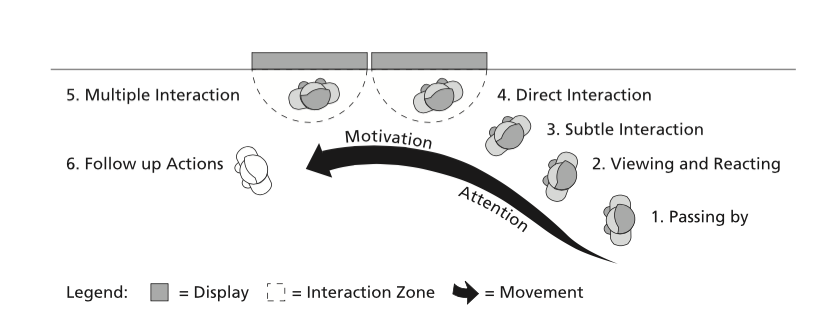
\includegraphics[width=120mm,height=70mm]{Figures/3/TheAudienceFunnel}
\caption{The Audience Funnel}
\label{fig:audience_funnel}
\end{figure}


\subsection{Interaction modalities}
\subsubsection{Body}
\subsubsection{Mobile}

\subsection{Interaction models}

\subsection{Evaluation}

\subsection{Approaches to Research}
\subsection{Methods and tools}







 





